\section{Hopf--Lax表示}
\label{sec:hj-hopf-lax}

比较原理保证黏性解至多一个，存在性还没有解决。对只依赖梯度的凸Hamilton量，解可以显式写出来，而且公式直接解释了尖点处选了哪一支。

\paragraph{从特征线到极小化}
设$H=H(\bm{p})$是凸函数，并且\term{超线性增长}（superlinear growth），即
\begin{equation}
  \lim_{\lVert\bm{p}\rVert_2\to\infty}\frac{H(\bm{p})}{\lVert\bm{p}\rVert_2}=+\infty.
  \label{eq:hj-superlinear}
\end{equation}
由第~\ref{sec:hj-characteristics}节的特征方程组，特征线是直线，斜率$\bm{p}$不变，速度$\bm{q}=\nabla H(\bm{p})$。沿线值的增量$\langle\bm{p},\nabla H(\bm{p})\rangle-H(\bm{p})$可以只用$\bm{q}$表示。

这里要用到凸共轭：对凸函数$H$，定义
\begin{equation}
  L(\bm{q})=\sup_{\bm{p}\in\mathbb{R}^{d}}\bigl\{\langle\bm{p},\bm{q}\rangle-H(\bm{p})\bigr\}.
  \label{eq:hj-legendre}
\end{equation}
$H$在$\bm{p}$处可微且$\bm{q}=\nabla H(\bm{p})$时，上确界在$\bm{p}$处取到，因此$L(\bm{q})=\langle\bm{p},\bm{q}\rangle-H(\bm{p})$，恰好是沿特征线值的增长率。凸共轭的基本性质（下半连续的凸函数共轭两次回到自身）可参考\BookChapterRef{chap:duality}{卷五第18章“对偶问题”}。

超线性让事情变得简单。对任意$r>0$，取$\bm{p}=r\bm{q}/\lVert\bm{q}\rVert_2$代入式~\eqref{eq:hj-legendre}，得到
\[
  L(\bm{q})\geq r\lVert\bm{q}\rVert_2-\max_{\lVert\bm{p}\rVert_2=r}H(\bm{p}).
\]
所以$L$同样超线性增长；由式~\eqref{eq:hj-superlinear}，式~\eqref{eq:hj-legendre}中的上确界有限。$L$是有限的凸函数，因而连续，并且由Fenchel--Moreau定理$H=L^*$。

最常用的例子是$H(\bm{p})=\lVert\bm{p}\rVert_2^2/2$，它的共轭是$L(\bm{q})=\lVert\bm{q}\rVert_2^2/2$。

从$\bm{y}$出发、时间$t$内到达$\bm{x}$的特征线速度是$\bm{q}=(\bm{x}-\bm{y})/t$，所以它带来的值是$u_0(\bm{y})+tL(\bm{q})$。不同的$\bm{y}$给出不同的候选值，我们取最小的一个。

\begin{definition}[Hopf--Lax公式]
\label{def:hj-hopf-lax}
设$H$凸且超线性增长，$L=H^*$，$u_0$有界且$R$-Lipschitz。对$t>0$，定义
\begin{equation}
  u(\bm{x},t)=\min_{\bm{y}\in\mathbb{R}^{d}}\Bigl\{u_0(\bm{y})+tL\Bigl(\frac{\bm{x}-\bm{y}}{t}\Bigr)\Bigr\},
  \label{eq:hj-hopf-lax}
\end{equation}
并令$u(\cdot,0)=u_0$。式~\eqref{eq:hj-hopf-lax}称为\term{Hopf--Lax公式}（Hopf--Lax formula）。
\end{definition}

对$H=p^2/2$，公式写成
\[
  u(x,t)=\min_y\Bigl\{u_0(y)+\frac{(x-y)^2}{2t}\Bigr\}.
\]
它有一个直观的图景，见图~\ref{fig:hj-parabola-touch}。把开口向下、顶点在$(x,c)$的抛物线$c-(x-y)^2/(2t)$放在$u_0$的下方，向上抬，直到碰到$u_0$，此时的$c$就是$u(x,t)$。接触点$y$是极小点，也就是这个位置的解“来自”的初始点。

\begin{BookInlineFigure}
  \centering
  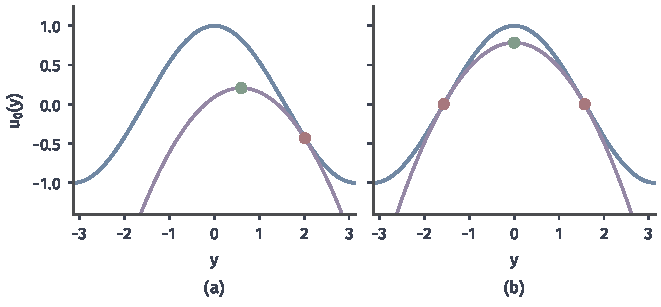
\includegraphics[width=112mm]{figures/06-differential-equations/02-partial-differential-equations/matplotlib/hj-parabola-touch/figure.pdf}
  \caption{Hopf--Lax公式的抛物线图景，$u_0=\cos y$（蓝），$t=\pi/2$。紫线是抬到碰上$u_0$为止的抛物线，绿点是顶点$(x,u(x,t))$，红点是接触点。(a)$x=0.6$，只有一个接触点。(b)$x=0$，两个接触点$y=\pm\pi/2$，顶点高度$\pi/4$。}
  \label{fig:hj-parabola-touch}
\end{BookInlineFigure}

\paragraph{公式的性质}
要证明式~\eqref{eq:hj-hopf-lax}给出黏性解，需要它的四条性质。最关键的一条是半群性质：走$t$时间等于先走$s$，再走$t-s$。

\begin{lemma}[Hopf--Lax公式的性质]
\label{lem:hj-hopf-lax}
在定义~\ref{def:hj-hopf-lax}的条件下：

(1)式~\eqref{eq:hj-hopf-lax}的极小值可以取到。

(2)$u(\cdot,t)$是$R$-Lipschitz的。

(3)对$0\leq s<t$，
\begin{equation}
  u(\bm{x},t)=\min_{\bm{y}}\Bigl\{u(\bm{y},s)+(t-s)L\Bigl(\frac{\bm{x}-\bm{y}}{t-s}\Bigr)\Bigr\}.
  \label{eq:hj-semigroup}
\end{equation}

(4)记
\begin{equation}
  C=\max\Bigl\{\lvert L(\bm{0})\rvert,\ \max_{\lVert\bm{p}\rVert_2\leq R}\lvert H(\bm{p})\rvert\Bigr\},
  \label{eq:hj-time-constant}
\end{equation}
则对$0\leq s\leq t$，
\begin{equation}
  \lvert u(\bm{x},t)-u(\bm{x},s)\rvert\leq C(t-s).
  \label{eq:hj-time-lipschitz}
\end{equation}
\end{lemma}

\begin{proof}
(1)括号内是$\bm{y}$的连续函数。$u_0$有界，$L$超线性增长，所以当$\lVert\bm{y}\rVert_2\to\infty$时括号内趋于$+\infty$，极小值可取到。

(2)设$\bm{y}$是$(\bm{x},t)$的极小点。把$\bm{y}+\hat{\bm{x}}-\bm{x}$代入$(\hat{\bm{x}},t)$的公式，$L$的自变量不变，所以
\[
  u(\hat{\bm{x}},t)-u(\bm{x},t)\leq u_0(\bm{y}+\hat{\bm{x}}-\bm{x})-u_0(\bm{y})\leq R\lVert\hat{\bm{x}}-\bm{x}\rVert_2.
\]
交换$\bm{x}$和$\hat{\bm{x}}$得到另一半。

(3)$s=0$时就是定义。设$s>0$。先证式中右端不超过左端。设$\bm{z}$是$(\bm{x},t)$的极小点，取线段上的点$\bm{y}=\frac{s}{t}\bm{x}+(1-\frac{s}{t})\bm{z}$，此时
\[
  \frac{\bm{x}-\bm{y}}{t-s}=\frac{\bm{y}-\bm{z}}{s}=\frac{\bm{x}-\bm{z}}{t}.
\]
用$u(\bm{y},s)\leq u_0(\bm{z})+sL((\bm{y}-\bm{z})/s)$，右端括号内不超过$u_0(\bm{z})+tL((\bm{x}-\bm{z})/t)=u(\bm{x},t)$。

再证左端不超过右端。任取$\bm{y}$，设$\bm{z}$是$(\bm{y},s)$的极小点。由$L$的凸性，
\[
  tL\Bigl(\frac{\bm{x}-\bm{z}}{t}\Bigr)\leq(t-s)L\Bigl(\frac{\bm{x}-\bm{y}}{t-s}\Bigr)+sL\Bigl(\frac{\bm{y}-\bm{z}}{s}\Bigr).
\]
再由$u(\bm{x},t)$的定义，得到
\[
  u(\bm{x},t)\leq u_0(\bm{z})+tL\Bigl(\frac{\bm{x}-\bm{z}}{t}\Bigr)\leq u(\bm{y},s)+(t-s)L\Bigl(\frac{\bm{x}-\bm{y}}{t-s}\Bigr).
\]

(4)先证$s=0$。上界由$\bm{y}=\bm{x}$得到：$u(\bm{x},t)\leq u_0(\bm{x})+tL(\bm{0})$。下界用$\bm{z}=(\bm{x}-\bm{y})/t$改写公式，再用Lipschitz条件：
\[
  u(\bm{x},t)\geq u_0(\bm{x})+t\min_{\bm{z}}\bigl\{L(\bm{z})-R\lVert\bm{z}\rVert_2\bigr\}.
\]
而$R\lVert\bm{z}\rVert_2$等于$\langle\bm{p},\bm{z}\rangle$在$\lVert\bm{p}\rVert_2\leq R$上的最大值。交换两个$\max$并用$H=L^*$，得到
\[
  -\min_{\bm{z}}\bigl\{L(\bm{z})-R\lVert\bm{z}\rVert_2\bigr\}=\max_{\lVert\bm{p}\rVert_2\leq R}H(\bm{p})\leq C.
\]
一般的$s$由式~\eqref{eq:hj-semigroup}和(2)，把$u(\cdot,s)$当作新的初值重复这一论证。
\end{proof}

\begin{theorem}[Hopf--Lax公式给出黏性解]
\label{thm:hj-hopf-lax}
在定义~\ref{def:hj-hopf-lax}的条件下，式~\eqref{eq:hj-hopf-lax}定义的$u$在任意$\mathbb{R}^{d}\times[0,t_{\mathrm{f}}]$上有界、Lipschitz，是初值问题$\partial_tu+H(\nabla u)=0$、$u(\cdot,0)=u_0$的黏性解，并且是有界、一致连续、关于$\bm{x}$为$R$-Lipschitz的函数类中唯一的黏性解。
\end{theorem}

\begin{proof}
由引理~\ref{lem:hj-hopf-lax}，$u$有界，界为$\sup\lvert u_0\rvert+Ct_{\mathrm{f}}$；$u$关于$\bm{x}$是$R$-Lipschitz的，关于$t$是$C$-Lipschitz的，$t=0$时取值$u_0$。

\emph{次解。}设$u-\varphi$在$(\bm{x}_0,t_0)$取局部极大，$t_0>0$。任取$\bm{q}$和小$h>0$，在式~\eqref{eq:hj-semigroup}中取$\bm{y}=\bm{x}_0-h\bm{q}$、$s=t_0-h$，得到
\[
  u(\bm{x}_0,t_0)\leq u(\bm{x}_0-h\bm{q},t_0-h)+hL(\bm{q}).
\]
由局部极大，$u-\varphi$在$(\bm{x}_0-h\bm{q},t_0-h)$处不大于在$(\bm{x}_0,t_0)$处，整理后得到
\[
  \varphi(\bm{x}_0,t_0)-\varphi(\bm{x}_0-h\bm{q},t_0-h)\leq hL(\bm{q}).
\]
除以$h$，令$h\to0$，得到
\[
  \partial_t\varphi+\langle\bm{q},\nabla\varphi\rangle-L(\bm{q})\leq0.
\]
对$\bm{q}$取上确界并用$H=L^*$，得到$\partial_t\varphi+H(\nabla\varphi)\leq0$。

\emph{上解。}设$u-\varphi$在$(\bm{x}_0,t_0)$取局部极小。由式~\eqref{eq:hj-semigroup}（取$s=t_0-h$）和(1)，存在$\bm{y}_h$，记$\bm{q}_h=(\bm{x}_0-\bm{y}_h)/h$，使
\[
  u(\bm{x}_0,t_0)=u(\bm{y}_h,t_0-h)+hL(\bm{q}_h).
\]
由$u$的Lipschitz性质，$hL(\bm{q}_h)\leq Rh\lVert\bm{q}_h\rVert_2+Ch$。$L$超线性增长，所以$\lVert\bm{q}_h\rVert_2$有不依赖$h$的上界。

由局部极小，同样整理得到
\[
  \varphi(\bm{x}_0,t_0)-\varphi(\bm{y}_h,t_0-h)\geq hL(\bm{q}_h).
\]
$\varphi\in C^1$且$\bm{q}_h$有界，所以左端等于$h(\partial_t\varphi+\langle\bm{q}_h,\nabla\varphi\rangle)+o(h)$，其中导数在$(\bm{x}_0,t_0)$处取值。除以$h$，得到
\[
  \partial_t\varphi+\langle\bm{q}_h,\nabla\varphi\rangle-L(\bm{q}_h)\geq o(1).
\]
由Fenchel--Young不等式（$H=L^*$的定义），左端第二、三两项不超过$H(\nabla\varphi)$。令$h\to0$，得到$\partial_t\varphi+H(\nabla\varphi)\geq0$。

\emph{唯一性。}$H$连续，在$\lVert\bm{p}\rVert_2\leq R$上一致连续，由定理~\ref{thm:hj-uniqueness}即得。
\end{proof}

证明的结构和方程的含义一一对应：极小化的上界对应每一条候选路线都给出不等式，所以次解成立；极小化取到的那条路线给出反向的不等式，所以上解成立。

\paragraph{公式怎样选择分支}
回到$u_0=\cos x$，取$t=\pi/2$、$x=0$。极小化的函数是$F(y)=\cos y+y^2/\pi$，临界点方程是
\[
  F'(y)=-\sin y+\frac{2y}{\pi}=0,
\]
即$\sin y=2y/\pi$。由$\sin$在$[0,\pi]$上的凹性，它的非负解只有$y=0$和$y=\pi/2$；再由对称性，全部解是$y=0,\pm\pi/2$。代入$F$得到
\[
  F(0)=1,\qquad F\bigl(\pm\tfrac{\pi}{2}\bigr)=\frac{\pi}{4}\approx0.785.
\]
所以$u(0,\pi/2)=\pi/4$，极小点是$y=\pm\pi/2$。这三个临界点恰好是第~\ref{sec:hj-cusps}节算出的三条特征线，函数值也与当时的$z$相同。

这个吻合有一般的原因。设$u_0$、$L$、$H$可微，$\bm{q}$表示$(\bm{x}-\bm{y})/t$，极小点满足一阶条件$\nabla u_0(\bm{y})=\nabla L(\bm{q})$。由共轭函数的性质，这等价于$\bm{q}$等于$\nabla H$在$\bm{p}_0=\nabla u_0(\bm{y})$处的值，也就是
\[
  \bm{x}=\bm{y}+t\nabla H(\bm{p}_0).
\]
所以每个临界点都对应一条到达$(\bm{x},t)$的特征线，临界值就是这条线带来的$z$。Hopf--Lax公式在所有特征线中选择取值最小的一条，这回答了第~\ref{sec:hj-cusps}节的问题：对凸的$H$，黏性解取的就是所有特征线候选的下包络。

图~\ref{fig:hj-argmin-jump}(a)是目标函数$F$。$x=0$时两个极小点等高；$x=0.3$时右侧变低，唯一的极小点约为$y=1.822$，极小值$0.489$。图(b)是极小点随$x$的变化，在$x=0$处从$-\pi/2$跳到$\pi/2$，这个跳跃就是图~\ref{fig:hj-cos-characteristics}(b)中两族特征线之间的分界。

\begin{BookInlineFigure}
  \centering
  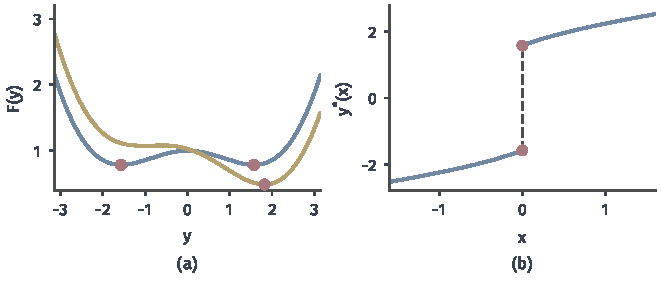
\includegraphics[width=112mm]{figures/06-differential-equations/02-partial-differential-equations/matplotlib/hj-argmin-jump/figure.pdf}
  \caption{极小点的跳跃，$t=\pi/2$，$F(y)=\cos y+(x-y)^2/(2t)$。(a)$x=0$（蓝）有两个等高的极小点，$x=0.3$（黄）只有一个，红点是极小点。(b)极小点$y^*(x)$，虚线处从$-\pi/2$跳到$\pi/2$。}
  \label{fig:hj-argmin-jump}
\end{BookInlineFigure}

\begin{theorem}[极小点决定梯度]
\label{thm:hj-minimizer-gradient}
设$L$连续可微，$\bm{y}$是$(\bm{x},t)$的一个极小点，$t>0$。若$u(\cdot,t)$在$\bm{x}$处可微，则
\begin{equation}
  \nabla u(\bm{x},t)=\nabla L\Bigl(\frac{\bm{x}-\bm{y}}{t}\Bigr).
  \label{eq:hj-minimizer-gradient}
\end{equation}
特别地，若$L$还是严格凸的，而$(\bm{x},t)$有两个不同的极小点，则$u(\cdot,t)$在$\bm{x}$处不可微。
\end{theorem}

\begin{proof}
对任意$\bm{x}'$，$\bm{y}$仍是公式的一个候选，所以
\[
  u(\bm{x}',t)\leq u_0(\bm{y})+tL\Bigl(\frac{\bm{x}'-\bm{y}}{t}\Bigr),
\]
且$\bm{x}'=\bm{x}$时取等。右端是$\bm{x}'$的$C^1$函数，从上方贴住$u(\cdot,t)$，一阶条件给出式~\eqref{eq:hj-minimizer-gradient}。

若有两个极小点，$(\bm{x}-\bm{y})/t$取两个不同的值，严格凸函数的梯度是单射，式~\eqref{eq:hj-minimizer-gradient}的右端不同，矛盾。
\end{proof}

不可微点就是多个极小点的位置，也就是特征线竞争时打平的位置。在$x=0$、$t=\pi/2$，两个极小点给出$q=(0\mp\pi/2)/(\pi/2)=\mp1$，$u$的左斜率是$+1$，右斜率是$-1$，形成凹折角。

折角只会是凹的，这一点可以直接证明。对$H=\lVert\bm{p}\rVert_2^2/2$，公式展开平方，得到
\[
  u(\bm{x},t)-\frac{\lVert\bm{x}\rVert_2^2}{2t}=\min_{\bm{y}}\Bigl\{u_0(\bm{y})+\frac{\lVert\bm{y}\rVert_2^2}{2t}-\frac{\langle\bm{x},\bm{y}\rangle}{t}\Bigr\}.
\]
右端是$\bm{x}$的仿射函数的极小，所以是凹函数。这种减去二次函数后变成凹函数的性质叫做\term{半凹}（semiconcave）。它排除了$t>0$时的一切凸折角。

一维时，这条性质说$\partial_xu-x/t$不增，即$v=\partial_xu$对$a>0$满足$v(x+a)-v(x)\leq a/t$。这就是Burgers方程熵解的单侧增长界（Oleinik条件），也说明了凹槽$w$的底部为何从一开始就被排除。

\paragraph{两种折角的算例}
把$u_0=\pm\lvert x\rvert$代入公式，可以完整地手算，取$H=p^2/2$。

对$u_0=\lvert x\rvert$，先在$y>0$上求极小：$1+(y-x)/t=0$，得$y=x-t$，要求$x>t$，此时值为$x-t/2$。$y<0$的情形对称。其余情况极小点在折角$y=0$处，值为$x^2/(2t)$。汇总得
\begin{equation}
  u(x,t)=\begin{cases}x^2/(2t),&\lvert x\rvert\leq t,\\\lvert x\rvert-t/2,&\lvert x\rvert>t.\end{cases}
  \label{eq:hj-convex-kink}
\end{equation}
初值的凸折角立刻被抹平。$\partial_xu=x/t$，正是第~\ref{chap:scalar-conservation-laws}章的稀疏波。

对$u_0=-\lvert x\rvert$，在$y>0$上一阶条件$-1+(y-x)/t=0$给出$y=x+t$，值$-x-t/2$；在$y<0$上$y=x-t$，值$x-t/2$。比较两者取较小，得到
\begin{equation}
  u(x,t)=-\lvert x\rvert-\frac{t}{2}.
  \label{eq:hj-concave-kink}
\end{equation}
凹折角一直存在，$x=0$上$v$的跳跃是激波。图~\ref{fig:hj-fan-kink}是两种情形的对比。

\begin{BookInlineFigure}
  \centering
  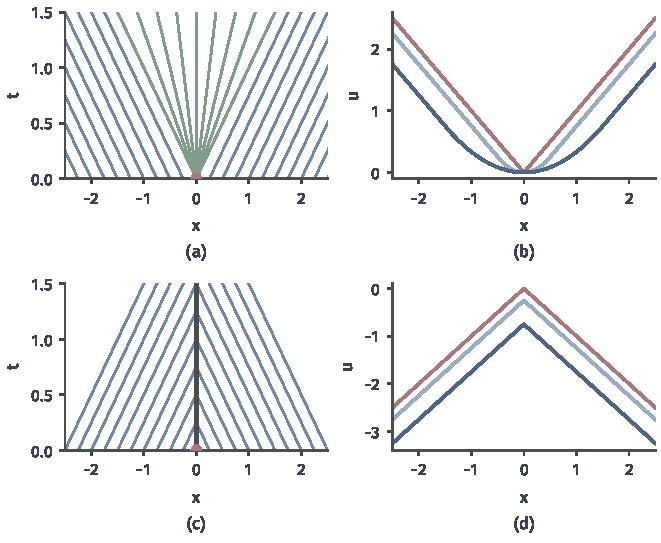
\includegraphics[width=112mm]{figures/06-differential-equations/02-partial-differential-equations/matplotlib/hj-fan-kink/figure.pdf}
  \caption{$H=p^2/2$下两种折角的演化。(a)、(b)$u_0=\lvert x\rvert$：折角处发出绿色扇形特征线填补空隙，解由式~\eqref{eq:hj-convex-kink}给出。(c)、(d)$u_0=-\lvert x\rvert$：蓝色特征线都汇入深灰的折角线，解由式~\eqref{eq:hj-concave-kink}给出。(b)、(d)中红线是初值，蓝色由浅到深是$t=0.5,1.5$。}
  \label{fig:hj-fan-kink}
\end{BookInlineFigure}

\paragraph{条件的作用}
凸性不能省略。公式只依赖$L=H^*$，而不同的$H$可能有相同的$L$。由Fenchel--Moreau定理，$L^*$是$H$的闭凸包，所以式~\eqref{eq:hj-hopf-lax}求解的其实是$H^{**}$对应的方程。若$H$不凸，$H^{**}\neq H$，公式给出的就不是原方程的解。

初值有界也用到了。对$u_0=-x^2/2$、$H=p^2/2$和$t>1$，公式中的目标函数
\[
  -\frac{y^2}{2}+\frac{(x-y)^2}{2t}
\]
的二次项系数是$\frac{1}{2t}-\frac12<0$，下确界是$-\infty$，公式失去意义。这和上一节经典解在$t=1$爆破是一致的。

\paragraph{到达时间：极限情形}
波前对应$H(\bm{p})=\lVert\bm{p}\rVert_2$，它是凸的，但只线性增长。此时共轭函数是单位球的指示函数：$\lVert\bm{q}\rVert_2\leq1$时$L(\bm{q})=0$，否则$L=+\infty$。把它代入式~\eqref{eq:hj-hopf-lax}，得到
\begin{equation}
  u(\bm{x},t)=\min_{\lVert\bm{y}-\bm{x}\rVert_2\leq t}u_0(\bm{y}).
  \label{eq:hj-erosion}
\end{equation}
定理~\ref{thm:hj-hopf-lax}不直接覆盖这种情形，但它的证明可以照搬：极小点在紧球上取得，半群性质只用到$L$的凸性，$\bm{q}_h$在单位球内，有界性不用再证，$H=L^*$仍然成立。所以式~\eqref{eq:hj-erosion}是有界Lipschitz初值下的黏性解。

这个公式说，$u$在$(\bm{x},t)$的值是初值在半径$t$的球内的最小值。取一个闭的源集$S$，$u_0=d(\cdot,S)$是到$S$的距离（要满足有界性，可以在远处截断，有限时间内的结果不受影响）。则
\[
  u(\bm{x},t)=\max\{d(\bm{x},S)-t,\ 0\},
\]
所以$\{u(\cdot,t)=0\}=\{d(\cdot,S)\leq t\}$恰好是时刻$t$已被扫过的区域，到达时间$T=d(\cdot,S)$从解中读出。

图~\ref{fig:hj-erosion}取一维的$S=\{-1.5,1\}$。相向的两列波前在$x=-0.25$、时刻$1.25$相遇，这正是图(b)的折角点。这与定理~\ref{thm:hj-distance}的结论一致，$T$就是到$S$的距离。

\begin{BookInlineFigure}
  \centering
  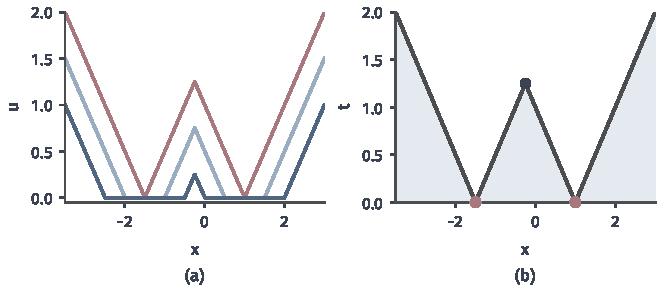
\includegraphics[width=112mm]{figures/06-differential-equations/02-partial-differential-equations/matplotlib/hj-erosion/figure.pdf}
  \caption{$H=\lvert p\rvert$的极限情形。(a)初值$u_0=d(x,S)$（红），$S=\{-1.5,1\}$，蓝色由浅到深是$t=0.5,1$的解，零值区域在扩大。(b)$(x,t)$平面，红点是源，深灰线是$T(x)=d(x,S)$，也就是四条波前的轨迹，浅蓝是波前尚未到达的区域$t<T(x)$，黑点$(-0.25,1.25)$是两列波前相遇的位置。}
  \label{fig:hj-erosion}
\end{BookInlineFigure}

Hopf--Lax公式的外形是在速度和代价之间做选择，让人想到控制问题。这一节只把它用作方程的表示公式：$L$由$H$算出来，极小化的作用是从特征线中选出黏性解。本章不需要问谁在做决策，也不需要讨论最优策略是否存在。
